\documentclass{beamer}

\pdfmapfile{+sansmathaccent.map}


\mode<presentation>
{
  \usetheme{Warsaw} % or try Darmstadt, Madrid, Warsaw, Rochester, CambridgeUS, ...
  \usecolortheme{seahorse} % or try seahorse, beaver, crane, wolverine, ...
  \usefonttheme{serif}  % or try serif, structurebold, ...
  \setbeamertemplate{navigation symbols}{}
  \setbeamertemplate{caption}[numbered]
} 


%%%%%%%%%%%%%%%%%%%%%%%%%%%%
% itemize settings

\definecolor{mypink}{RGB}{255, 150, 150}
\definecolor{myblue}{RGB}{150, 150, 255}
\definecolor{mygray}{gray}{0.8}

\setbeamertemplate{itemize items}[default]

\setbeamertemplate{itemize item}{\color{mypink}$\blacksquare$}
\setbeamertemplate{itemize subitem}{\color{myblue}$\blacktriangleright$}
\setbeamertemplate{itemize subsubitem}{\color{mygray}$\blacksquare$}

%%%%%%%%%%%%%%%%%%%%%%%%%%%%
% block settings

\setbeamercolor{block title}{bg=red!30,fg=black}


%%%%%%%%%%%%%%%%%%%%%%%%%%%%
% URL settings
\hypersetup{
    colorlinks=true,
    linkcolor=blue,
    filecolor=blue,      
    urlcolor=blue,
}

%%%%%%%%%%%%%%%%%%%%%%%%%%

\renewcommand{\familydefault}{\rmdefault}

\usepackage{amsmath}
\usepackage{mathtools}

\DeclareMathOperator*{\argmin}{arg\,min}

\usepackage{subcaption}




%%%%%%%%%%%%%%%%%%%%%%%%%%%%
% code settings

\usepackage{listings}
\usepackage{color}
\definecolor{mygreen}{rgb}{0,0.6,0}
\definecolor{mygray}{rgb}{0.5,0.5,0.5}
\definecolor{mymauve}{rgb}{0.58,0,0.82}
\lstset{ 
  backgroundcolor=\color{white},   % choose the background color; you must add \usepackage{color} or \usepackage{xcolor}; should come as last argument
  basicstyle=\footnotesize,        % the size of the fonts that are used for the code
  breakatwhitespace=false,         % sets if automatic breaks should only happen at whitespace
  breaklines=true,                 % sets automatic line breaking
  captionpos=b,                    % sets the caption-position to bottom
  commentstyle=\color{mygreen},    % comment style
  deletekeywords={...},            % if you want to delete keywords from the given language
  escapeinside={\%*}{*)},          % if you want to add LaTeX within your code
  extendedchars=true,              % lets you use non-ASCII characters; for 8-bits encodings only, does not work with UTF-8
  firstnumber=0000,                % start line enumeration with line 0000
  frame=single,	                   % adds a frame around the code
  keepspaces=true,                 % keeps spaces in text, useful for keeping indentation of code (possibly needs columns=flexible)
  keywordstyle=\color{blue},       % keyword style
  language=Octave,                 % the language of the code
  morekeywords={*,...},            % if you want to add more keywords to the set
  numbers=left,                    % where to put the line-numbers; possible values are (none, left, right)
  numbersep=5pt,                   % how far the line-numbers are from the code
  numberstyle=\tiny\color{mygray}, % the style that is used for the line-numbers
  rulecolor=\color{black},         % if not set, the frame-color may be changed on line-breaks within not-black text (e.g. comments (green here))
  showspaces=false,                % show spaces everywhere adding particular underscores; it overrides 'showstringspaces'
  showstringspaces=false,          % underline spaces within strings only
  showtabs=false,                  % show tabs within strings adding particular underscores
  stepnumber=2,                    % the step between two line-numbers. If it's 1, each line will be numbered
  stringstyle=\color{mymauve},     % string literal style
  tabsize=2,	                   % sets default tabsize to 2 spaces
  title=\lstname                   % show the filename of files included with \lstinputlisting; also try caption instead of title
}

%%%%%%%%%%%%%%%%%%%%%%%%%%%%
% tikz settings

\usepackage{tikz}
\tikzset{every picture/.style={line width=0.75pt}}


\title{Solving Mechanical Equations with Constraints}
\subtitle{Contact-aware Control, Lecture 5}
\author{by Sergei Savin}
\centering
\date{Fall 2020}



\begin{document}
\maketitle


\begin{frame}{Content}

\begin{itemize}
\item Solving first order ODEs
\item Solving second order ODEs
\item Mechanical equations
\item Mechanical equations with constraints
\item Constraint drift
\begin{itemize}
\item Part 1: right-hand-side
\item Part 2-3: velocities
\item Part 4-6: positions
\end{itemize}
\item Read more
\item Homework
\end{itemize}

\end{frame}



\begin{frame}{Solving first order ODEs}
% \framesubtitle{O}
\begin{flushleft}

General form first order ODE has the form:

\begin{equation}
\label{eq:simple_ODE}
\dot{\bo{x}} = \bo{f}(\bo{x}, t)
\end{equation}

Solving it, means finding such $\bo{x}(t)$ that eq. \eqref{eq:simple_ODE} becomes equality. A typical strategy for solving it is a "forward" scheme, for example:

\begin{equation}
\label{eq:Euler_scheme}
\bo{x}_{i+1} = \bo{x}_i + \bo{f}(\bo{x}_i, t) \Delta t
\end{equation}

which is called forward Euler scheme. Backward (implicit) scheme would only be different in the function $\bo{f}$ being evaluated at the point $\bo{x}_{i+1}$: $\bo{f}(\bo{x}_{i+1}, t)$ Other famous schemes are Runge-Kutta, variable step schemes, etc.

\end{flushleft}
\end{frame}




\begin{frame}{Solving second order ODEs}
% \framesubtitle{O}
\begin{flushleft}

Second order ODE have the form:

\begin{equation}
\label{eq:secondOrderODE}
\ddot{\bo{x}} = \bo{g}(\dot{\bo{x}}, \bo{x}, t)
\end{equation}

\begin{block}{Observation 1}
Every second order differential equation expressed in the normal form can be re-expressed as a system of first order ODEs.
\end{block}

But we don't have to go this rout. Instead we can, for example, use Taylor expansion to solve the equations:

\begin{equation}
\label{eq:Taylor_scheme}
\begin{cases}
\dot{\bo{x}}_{i+1} = \dot{\bo{x}}_i + \bo{g}(\dot{\bo{x}}_i, \bo{x}_i, t) \Delta t \\
\bo{x}_{i+1} = \bo{x}_i + \dot{\bo{x}}_i \Delta t + 0.5 \bo{g}(\dot{\bo{x}}_i, \bo{x}_i, t) \Delta t^2
\end{cases}
\end{equation}

\end{flushleft}
\end{frame}




\begin{frame}{Mechanical equations}
% \framesubtitle{O}
\begin{flushleft}

Consider this special form of second order differential equations:

\begin{equation}
\bo{H} \ddot{\bo{q}} + \bo{c} = \tau
\end{equation}

First thing you can do is to rewrite it in the form where higher order derivatives are collected on the left hand side:

\begin{equation}
\ddot{\bo{q}} = \bo{H}^{-1} (\tau - \bo{c})
\end{equation}

Notice that for mechanical systems $\bo{H}$ is always invertible. Prove it, using the fact $\bo{H}$ is the quadratic form matrix of the kinetic energy:  $T = 0.5 \dot{\bo{q}}^\top\bo{H}\dot{\bo{q}}$

\bigskip

Next we either turn it into a system of first order ODEs and solve it using methods for those, or leave it a second order ODE and solve it, for example, using \eqref{eq:Taylor_scheme}.

\end{flushleft}
\end{frame}


\begin{frame}{Mechanical equations with constraints}
\framesubtitle{Part 1}
\begin{flushleft}

Now, how do we solve this system of equations?

\begin{equation}
\begin{cases}
    \bo{H} \ddot{\bo{q}} + \bo{c} = \tau + \bo{F}^\top \lambda \\
    \bo{g}(\bo{q}) = 0
\end{cases}
\end{equation}

Notice there are two unknown: $\bo{q}$ and $\lambda$. One has a second order derivative, another one is an algebraic variable. Also, notice that the first vector equation in the case includes derivatives, while the other does not. Equations like this are called DAE - \emph{differential algebraic equations}.

\bigskip

There are a number of methods of solving DAE, but when one of the equation is algebraic, the rule of thumb is to differentiate it first, so we can use it in finding higher order derivatives.

\end{flushleft}
\end{frame}



\begin{frame}{Mechanical equations with constraints}
\framesubtitle{Part 2}
\begin{flushleft}

After differentiating $\bo{g}(\bo{q}) = 0$ twice, and defining $\bo{F} = \frac{\partial \bo{g}}{\partial \bo{q}}$, we get:

\begin{equation}
\begin{cases}
    \bo{H} \ddot{\bo{q}} + \bo{c} = \tau + \bo{F}^\top \lambda \\
    \bo{F} \ddot{\bo{q}} + \dot{\bo{F}} \dot{\bo{q}} = 0
\end{cases}
\end{equation}

Now we can treat both $\ddot{\bo{q}}$ and $\lambda$ as unknown algebraic variables, and solve for them. This leads to a system:

\begin{equation}
\begin{bmatrix}
    \bo{H} & -\bo{F}^\top \\
    \bo{F} & \bo{0}
\end{bmatrix}
\begin{bmatrix}
    \ddot{\bo{q}} \\
    \lambda
\end{bmatrix}
=
\begin{bmatrix}
    \tau - \bo{c} \\
    -\dot{\bo{F}} \dot{\bo{q}}
\end{bmatrix}
\end{equation}

Matrix on the left hand side is invertible, as long as the reaction forces are uniquely defined (in other words, as long as $\bo{F}^\top$ has a trivial null space).

\end{flushleft}
\end{frame}



\begin{frame}{Mechanical equations with constraints}
\framesubtitle{Part 3}
\begin{flushleft}

Let us define $\bo{M} = \begin{bmatrix}
    \bo{H} & -\bo{F}^\top \\
    \bo{F} & \bo{0}
\end{bmatrix}$. Assuming that you found left inverse of $\bo{M}$ - let us call it matrix $\bo{L}$, $\bo{L}\bo{M} = \bo{I}$ - you write expressions for both $\ddot{\bo{q}}$ and $\lambda$ in terms of its components:

\begin{equation}
\label{eq:normal_form_DAE}
    \begin{cases}
        \ddot{\bo{q}} = 
        \bo{L}_{11} ( \tau - \bo{c}) - \bo{L}_{12} \dot{\bo{F}} \dot{\bo{q}} \\ 
        \lambda = \bo{L}_{21} ( \tau - \bo{c}) - \bo{L}_{22} \dot{\bo{F}} \dot{\bo{q}}
    \end{cases}
\end{equation}

This is useful both for simulation and for getting an insight into the dynamical system behaviour. 

\end{flushleft}
\end{frame}





\begin{frame}{Constraint drift}
\framesubtitle{Part 1}
\begin{flushleft}

If we simply integrate the \eqref{eq:normal_form_DAE}, the error will gradually accumulate and values of $\dot{\bo{q}}$ and $\bo{q}$ will drift, even as $\ddot{\bo{q}}$ is calculated precisely.

\bigskip

There are a number of techniques for fixing the constraint drift. Here we will see how to use projection onto the constraint manifold to minimize the drift in the direction, violating constraints. Constraint manifold here is:

\begin{equation}
\begin{cases}
    \bo{g}(\bo{q}) = 0 \\
    \bo{F} \dot{\bo{q}} = 0
\end{cases}
\end{equation}

\end{flushleft}
\end{frame}





\begin{frame}{Constraint drift}
\framesubtitle{Part 2 - velocities}
\begin{flushleft}

Let us consider the velocity constraint equation $\bo{F} \dot{\bo{q}} = 0$. All solutions to this equation are found in the form:

\begin{equation}
    \dot{\bo{q}} = \bo{N}\bo{z}
\end{equation}

where $\bo{N} = \text{null}(\bo{F})$ - null space of the matrix $\bo{F}$, and $\bo{z}$ are parameters in the minimal coordinate representation (encoding) of the null space solution for this linear system. 


\end{flushleft}
\end{frame}





\begin{frame}{Constraint drift}
\framesubtitle{Part 3 - velocities}
\begin{flushleft}


We need to solve the following optimization:

\begin{equation}
\begin{aligned}
& \underset{\bo{z}, \dot{\bo{q}}}{\text{minimize}}
& & || \dot{\bo{q}}_e - \dot{\bo{q}} || \\
& \text{subject to}
& & \dot{\bo{q}} = \bo{N}\bo{z}
%
\end{aligned}
\end{equation}

where $\dot{\bo{q}}_e$ is the estimate of of the generalized velocity, possibly containing the drift.

\bigskip

Substituting, we acquire a simple least squares problem of minimizing $||\dot{\bo{q}}_e - \bo{N}\bo{z}||$, whose solution is $\bo{z} = \bo{N}^+\dot{\bo{q}}_e$. Final solution is:

\begin{equation}
    \dot{\bo{q}} = \bo{N}\bo{N}^+\dot{\bo{q}}_e
\end{equation}

We can recognize it as a simple projection of the estimate $\dot{\bo{q}}_e$ onto the column space of $\bo{N}$.

\end{flushleft}
\end{frame}





\begin{frame}{Constraint drift}
\framesubtitle{Part 4 - positions}
\begin{flushleft}


Now we can consider position. Equation $\bo{g}(\bo{q}) = 0$ is non-linear, so we can use Taylor expansion on it:

\begin{equation}
    \bo{g}(\bo{q}) \sim \bo{g}_0 + \bo{F} (\bo{q} - \bo{q}_0) 
\end{equation}

where $\bo{q}_0$ is the linearization point; you can choose the current position estimate $\bo{g}_e$ or the current desired position or anything else. Be aware that your choice will affect your solution.

\bigskip

General solution to the equation $\bo{g}_0 + \bo{F} (\bo{q} - \bo{q}_0) = 0$ is:

\begin{equation}
    \bo{q} =  \bo{q}_0 - \bo{F}^+\bo{g}_0 + \bo{N}\zeta
\end{equation}

where $\zeta$ serves the same role as $\bo{z}$ did previously, except for positions.

\end{flushleft}
\end{frame}




\begin{frame}{Constraint drift}
\framesubtitle{Part 5 - positions}
\begin{flushleft}


We need to solve the following optimization to fix position drift:

\begin{equation}
\begin{aligned}
& \underset{\zeta, \bo{q}}{\text{minimize}}
& & || \bo{q}_e - \bo{q} || \\
& \text{subject to}
& & \bo{q} =  \bo{q}_0 - \bo{F}^+\bo{g}_0 + \bo{N}\zeta
%
\end{aligned}
\end{equation}

Same as before, we get a least-squares problem of minimizing $|| \bo{q}_e - \bo{q}_0 + \bo{F}^+\bo{g}_0 - \bo{N}\zeta ||$, with the solution $\zeta = \bo{N}^+(\bo{q}_e - \bo{q}_0 + \bo{F}^+\bo{g}_0)$. Finally, the expression for the fixed position is:

\begin{equation}
   \bo{q}  = \bo{q}_0 - \bo{F}^+\bo{g}_0 + \bo{N}\bo{N}^+(\bo{q}_e - \bo{q}_0 + \bo{F}^+\bo{g}_0)
\end{equation}

and after collecting the terms:

\begin{equation}
   \bo{q}  = (\bo{I} - \bo{N}\bo{N}^+) (\bo{q}_0 - \bo{F}^+\bo{g}_0) + \bo{N}\bo{N}^+\bo{q}_e
\end{equation}

\end{flushleft}
\end{frame}




\begin{frame}{Constraint drift}
\framesubtitle{Part 6 - positions}
\begin{flushleft}

We can recognize that this expression:

\begin{equation}
   \bo{q}  = (\bo{I} - \bo{N}\bo{N}^+) (\bo{q}_0 - \bo{F}^+\bo{g}_0) + \bo{N}\bo{N}^+\bo{q}_e
\end{equation}

is a projection of the particular solution $\bo{q}_0 - \bo{F}^+\bo{g}_0$ onto the left null space of $\bo{N}$ and of the initial estimate $\bo{q}_e$ onto the column space of $\bo{N}$.

\bigskip

All these projections can be achieved with a single SVD decomposition of the matrix $\bo{F}$ to find $\bo{N}$, since $\bo{N}$ is orthonormal and its pseudoinverse is equivalent to its transpose.

\end{flushleft}
\end{frame}




\begin{frame}{Read more}
% \framesubtitle{Parameter estimation}
\begin{flushleft}

You can read more about Lagrange equation derivation at:

\begin{itemize}
    \item \href{https://idp.springer.com/authorize/casa?redirect_uri=https://link.springer.com/content/pdf/10.1007/BF01385770.pdf&casa_token=Qba9ilJAgVkAAAAA:qXdlKw8Au9f4ZzDqbNKCo5dg5q_vFeQVVCHqbshd1rmld1nKTUoaCzZR-w_SfgQYL9d_GqfhYZOyn5RpZw}{Führer, C. and Leimkuhler, B.J., 1991. Numerical solution of differential-algebraic equations for constrained mechanical motion. Numerische Mathematik, 59(1), pp.55-69.} - read to get the feeling of the field.
\end{itemize}

\end{flushleft}
\end{frame}


\begin{frame}{Homework}
% \framesubtitle{Parameter estimation}
\begin{flushleft}

Simulate the motion of this robot forward (description of the robot is given in the previous lectures).

\begin{figure}
    \centering
    


\tikzset{every picture/.style={line width=0.75pt}} %set default line width to 0.75pt        

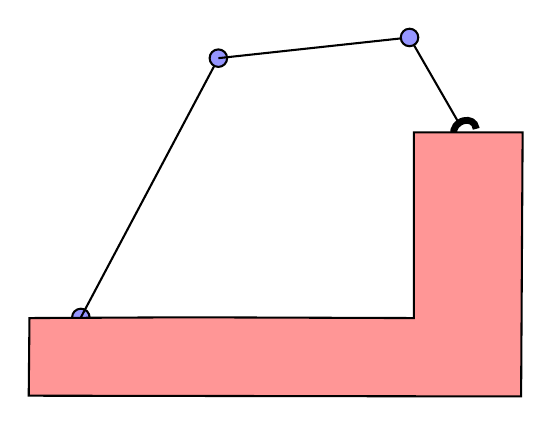
\begin{tikzpicture}[x=0.55pt,y=0.55pt,yscale=-1,xscale=1]
%uncomment if require: \path (0,300); %set diagram left start at 0, and has height of 300

%Shape: Circle [id:dp2680036705913309] 
\draw  [fill=myblue  ,fill opacity=1 ] (144.5,190.35) .. controls (144.5,187.17) and (147.07,184.6) .. (150.25,184.6) .. controls (153.43,184.6) and (156,187.17) .. (156,190.35) .. controls (156,193.53) and (153.43,196.1) .. (150.25,196.1) .. controls (147.07,196.1) and (144.5,193.53) .. (144.5,190.35) -- cycle ;
%Straight Lines [id:da511009501867824] 
\draw    (150.25,190.35) -- (240.6,20) ;
%Shape: Circle [id:dp33456176340238253] 
\draw  [fill=myblue  ,fill opacity=1 ] (234.85,20) .. controls (234.85,16.82) and (237.42,14.25) .. (240.6,14.25) .. controls (243.78,14.25) and (246.35,16.82) .. (246.35,20) .. controls (246.35,23.18) and (243.78,25.75) .. (240.6,25.75) .. controls (237.42,25.75) and (234.85,23.18) .. (234.85,20) -- cycle ;
%Straight Lines [id:da8106680503102979] 
\draw    (240.6,20) -- (366.2,6.4) ;
%Straight Lines [id:da7152287278059997] 
\draw    (399.4,64) -- (366.2,6.4) ;
%Shape: Circle [id:dp1080265764134869] 
\draw  [fill=myblue  ,fill opacity=1 ] (360.45,6.4) .. controls (360.45,3.22) and (363.02,0.65) .. (366.2,0.65) .. controls (369.38,0.65) and (371.95,3.22) .. (371.95,6.4) .. controls (371.95,9.58) and (369.38,12.15) .. (366.2,12.15) .. controls (363.02,12.15) and (360.45,9.58) .. (360.45,6.4) -- cycle ;
%Shape: Block Arc [id:dp8677516838116468] 
\draw  [fill={rgb, 255:red, 0; green, 0; blue, 0 }  ,fill opacity=1 ] (397.16,75.17) .. controls (396.21,74.66) and (395.39,73.93) .. (394.76,73.02) .. controls (392.25,69.38) and (393.66,64.05) .. (397.92,61.11) .. controls (402.18,58.16) and (407.67,58.73) .. (410.18,62.36) .. controls (410.82,63.28) and (411.2,64.3) .. (411.35,65.37) -- (408.23,66.19) .. controls (408.19,65.47) and (407.96,64.78) .. (407.55,64.18) .. controls (406.04,62) and (402.55,61.8) .. (399.74,63.74) .. controls (396.94,65.68) and (395.88,69.02) .. (397.39,71.2) .. controls (397.8,71.8) and (398.37,72.25) .. (399.02,72.54) -- cycle ;
%Shape: Polygon [id:ds12621320375323086] 
\draw  [fill=mypink  ,fill opacity=1 ] (440.5,68.75) -- (369,68.75) -- (369,190.75) -- (219.5,190.25) -- (116.5,190.75) -- (116,241.75) -- (439.5,242.25) -- cycle ;




\end{tikzpicture}

    %\caption{Caption}
    %\label{fig:my_label}
\end{figure}

\end{flushleft}
\end{frame}



\begin{frame}
\centerline{Lecture slides are available via Moodle.}
\bigskip
\centerline{You can help improve these slides at:}
\centerline{\href{https://github.com/SergeiSa/Contact-Aware-Control-Slides-Fall-2020}{github.com/SergeiSa/Contact-Aware-Control-Slides-Fall-2020}}
\bigskip
\centerline{Check Moodle for additional links, videos, textbook suggestions.}
\end{frame}

\end{document}
